\documentclass{article}

\usepackage[T1]{fontenc}    %Schriftart des Dokumentes
\usepackage[ngerman]{babel} %Dokumentensprache, hier Deutsch
\usepackage{amsmath, amssymb, stmaryrd} %mathematische Schriftzeichen
\usepackage{graphicx} %Einfügen von Grafiken
\usepackage{wrapfig}
\usepackage{bm}
\usepackage{subfig}
\usepackage{newclude}
\usepackage{pdfpages}
\usepackage{booktabs}

\setlength{\parindent}{0pt} %Einrückung von Absätzen auf null gesetzt
\setlength{\parskip}{10pt} %Abstand zischen Absätzen auf 10pt gesetzt

\title{Versuch 223: Brownsche Bewegung}
\author{Matthias Kuntz}
\date{06.03.2024}

\renewcommand*\contentsname{Zusammenfassung}

\begin{document}

\maketitle

\tableofcontents

\newpage

%-------------------------EINLEITUNG-------------------------
\section{Einleitung}

Mit die wohl wichtigsten physikalischen Erkenntnisse zu Beginn des 20. Jahrhunderts waren die Existenz von Atomen und Molekülen sowie die darauf basierenden Erfolge der Forschung in der Thermodynamik. Die Erforschung der Bewegung der Moleküle im Kontext der Theorie der Wärme und die darauffolgende experimentelle Bestätigung der in diesem Versuch betrachteten Brownschen Bewegung waren sogar Grund für die Verleihung des Physik-Nobelpreises im Jahr 1926. Die Brownsche Bewegung beschreibt die zufälligen Bewegungen kleiner Teilchen in einer Flüssigkeit, basierend auf vielen fortwährenden Stößen der Teilchen mit den Fluidmolekülen. Um dieses Phänomen zu untersuchen, wollen wir in diesem Versuch winzige Latexkügelchen in Wasser unter einem Mikroskop beobachten, wobei die Brownsche Bewegung sichtbar wird. Aus der quantitaviten Auswertung dieser Bewegung lässt sich im Endeffekt die Boltzmann-Konstante bestimmen.


\subsection{Physikalische Grundlagen}

\subsubsection{Das Random-Walk-Modell}

Ein Modell zur effektiven Beschreibung der Brownschen Bewegung ist der sogenannte Random-Walk. Um das System erstmal grundlegend zu verstehen möchten wir zunächst den einfachsten Fall betrachten: Ein Teilchen, das sich eindimensional entlang einer Achse entweder nach links oder nach rechts bewegen kann, so wie in Abbildung \ref{fig:randomwalk} dargestellt.

\begin{figure}[!h]
    \centering
    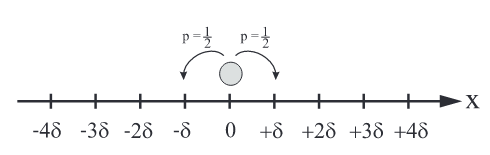
\includegraphics[width=0.7\textwidth]{graphics/randomwalk.png}
    \caption{Eindimensionaler Random-Walk [Quelle: PAP2.1 Skript, S.52, 08.03.2024]}
    \label{fig:randomwalk}
\end{figure}

Man setzt das Teilchen an eine Startposition, hier $x = 0$, und lässt dieses nun in regelmäßigen Abständen $\tau$ immer einen gleich großen Schritt $\delta$ in eine zufällig ausgewählte Richtung gehen. Dabei geht man davon aus, dass die Wahrscheinlichkeit $p$ für beide Richtungen gleich groß ist. Somit gilt, dass man nach einer Zeit $t$ exakt $n = t/\tau$ Stoßprozesse beobachtet. Machen wir nun noch die Annahme, dass die Bewegung eines Teilchens beim Random-Walk komplett unabhängig von allen anderen möglicherweise vorhandenen Teilchen ist, was vor allem im Kontext der Brownschen Bewegung, wo immer mehrere Teilchen vorhanden sein werden, wichtig ist, so können wir nun mit diesen Grundlagen die Wahrscheinlichkeit ermitteln mit der sich ein Teilchen nach einer gewissen Zeit $t$ im Intervall [$x$, $x+\Delta x$] befindet:

Dazu benötigen wir zunächst die folgende Erkenntnis: Um das Teilchen nach $n$-Stößen genau an der Position $x = m \delta$ zu finden, so muss dieses exakt $(n+m)/2$-mal nach rechts und $(n-m)/2$-mal nach links gelaufen sein. Später relevant wird auch die Beobachtung, dass $m$ bei geraden $n$ ebenfalls gerade und bei ungeraden $n$ analog ebenfalls ungerade sein muss. 
Es gibt nun wie aus der Wahrscheinlichkeitsrechnung bekannt mehrere Wege, wie das Teilchen die Endposition erreicht. Beispielsweise könnte es zuerst alle Schritte in positive und dann alle in negative oder immer abwechselnd in verschiedene Richtungen gehen. Somit lässt sich folgendermaßen berechnen, wie viele Möglichkeiten es gibt nach $n$ Schritten die Position $m$ zu erreichen:

\begin{equation}
    \binom{n}{\frac{1}{2}(n+m)} = \frac{n!}{[\frac{1}{2}(n+m)]! [\frac{1}{2}(n-m)]!}.
\end{equation}

Mit der Binomialverteilung ergibt sich die zugehörige Wahrscheinlichkeit $P(m;n)$, wobei wir direkt mit $p=\frac{1}{2}$ vereinfachen, da die Wahrscheinlichkeit in beide Richtungen gleich groß ist:

\begin{equation}
    \begin{split}
        P(m;n) &= \binom{n}{\frac{1}{2}(n+m)} \ p^{\frac{1}{2}(n+m)} \ (1-p)^{\frac{1}{2}(n-m)} \\
        \overset{p = \frac{1}{2}}{\Rightarrow} P(m;n) &= \frac{n!}{[\frac{1}{2}(n+m)]! [\frac{1}{2}(n-m)]!} \left( \frac{1}{2} \right)^n.
    \end{split}
\end{equation}

\subsubsection{Vereinfachungen für die Brownsche Bewegung}

Bei der Brownschen Bewegung passieren in der Regel sehr viele Stöße in kurzer Zeit, ergo $\tau$ ist sehr klein und $n=t/\tau$ wird bereits bei einer Beobachtungszeit von $t=1$s sehr groß. Diese Erkenntnis ermöglicht uns $n!$ und $m!$ mit der Stirling Formel zu nähern:

\begin{equation}
    n! = (2 \pi n)^\frac{1}{2} n^n e^{-n}.
\end{equation}

Somit erhalten wir nach einigen Unformungen die Wahrscheinlichkeit

\begin{equation}
    P(m;n) = \sqrt{\frac{2}{\pi n}} \exp{\left( - \frac{m^2}{2n} \right)}.
\end{equation}

Nun ist es angebracht, $n$ und $m$ durch die bei der Brwonschen Bewegung besser messbaren Größen $x$ und $t$ zu substituieren. Dabei erinnern wir uns zurück, dass $m$ entweder gerade oder ungerade ist und somit $\Delta m = \pm 2$ gilt, woraus unmittelbar

\begin{equation}
    P(m;n) \frac{\Delta x}{2 \delta} = P(x;n) \Delta x
\end{equation}

folgt und wir nach den Substitutionen $n = t/\tau$ sowie $m = x/\delta$ die Wahrscheinlichkeit erhalten, ein Teilchen nach der Zeit $t$ im Bereich [$x$, $x+\Delta x$] zu finden. Wir definieren zusätzlich die Größe $D = \delta^2 / 2 \tau$, deren physikalische Bedeutung später relevant wird. 

\begin{equation}
    P(x;t) \Delta x = \frac{\Delta x}{\sqrt{4 \pi D t}} \ \exp{\left( - \frac{x^2}{4Dt} \right)}.
\end{equation}

Bei genauerer Betrachtung fällt auf, dass dies genau der Form einer Gaußverteilung entspricht. Diese haben die allgemeine Form

\begin{equation}
    G(x; \mu, \sigma) = \frac{1}{\sqrt{2 \pi} \sigma} \ \exp{\left( - \frac{(x-\mu)^2}{2\sigma^2} \right)}
\end{equation}

mit den Größen des Mittelwerts $\mu$ sowie der Varianz $\sigma^2$ beziehungsweise der Standardabweichung $\sigma$. Da Gaußverteilungen allgemein symmetrisch um den Mittelwert sind, ist dieser sogleich der Erwartungswert $\langle x \rangle$. Angewendet auf unsere Wahrscheinlichkeitsverteilung der Brownschen Bewegung ergibt sich somit für mit mittlere Verrückung:

\begin{equation}
    \langle x \rangle = \int_{-\infty}^\infty x \ P(x;t) \ dx = 0.
\end{equation}

Somit enthält der Mittelwert $\langle x \rangle$ keine Informationen über die Bewegung des Teilchens und hilft uns somit hier nicht weiter. Daher betrachten wir stattdessen das mittlere Verschiebungsquadrat $\langle x^2 \rangle$:

\begin{equation}
    \langle x^2 \rangle = \int_{-\infty}^\infty x^2 \ P(x;t) \ dx = 2Dt = \sigma^2.
\end{equation}

Somit erkennen wir, dass das mittlere Verschiebungsquadrat gleich der Varianz ist und wir erhalten als erstes wichtiges Ergebnis die Einstein-Smoluchowski-Gleichung:

\begin{equation}
    \sqrt{\langle x^2 \rangle} = \sqrt{2Dt}.
\end{equation}

\subsubsection{Die Brownsche Bewegung in mehreren Dimensionen}

Soeben haben wir den vereinfachten Fall einer Brownschen Bewegung in einer Dimension mithilfe des Random-Walk-Modells hergeleitet. Geht man nun in beispielsweise zwei Dimensionen über, so gilt für das mittlere Verschiebungsquadrat, welches nun mit $\langle r^2 \rangle$ bezeichnet wird:

\begin{equation}
    \langle r^2 \rangle = \langle x^2 \rangle + \langle y^2 \rangle.
\end{equation}

Dabei ist die Brownsche Bewegung isotrop, ergo in alle Raumrichtungen uniform, wodurch jeder Term den Beitrag $2Dt$ liefert und somit für zwei Dimensionen

\begin{equation}
    \sqrt{\langle r^2 \rangle} = \sqrt{4Dt}
    \label{eq:r^2_2dim}
\end{equation}

beziehungsweise drei Dimensionen

\begin{equation}
    \sqrt{\langle r^2 \rangle} = \sqrt{6Dt}
\end{equation}

gilt. Es ist nun auch angebracht, die vorhin etwas willkürlich eingeführte Größe $D$ zu erklären: $D$ bezeichnet den sogenannten Diffusionskoeffizient und ist ein Maß für die Beweglichkeit eines Partikels in dem umgebenden Medium. Hierbei definierte Einstein die Form

\begin{equation}
    D = \frac{k_B T}{f},
\end{equation}

wobei $f$ den Reibungskoeffizienten, $k_B$ die Boltzmann-Konstante und $T$ die Temperatur der Flüssigkeit darstellen. Mit dem Stokes'schen Gesetz $f = 6 \pi \eta a$ für kugelförmige Partikel des Radius $a$ in einer Flüssigkeit mit Viskosität $\eta$ ergibt sich die Form des Diffusionskoeffizienten nach Einstein-Stokes:

\begin{equation}
    D = \frac{k_B T}{6 \pi \eta a}.
    \label{eq:Einst_Stokes_D}
\end{equation}

Setzt man diese Form in Gleichung \ref{eq:r^2_2dim} ein, so erhält man eine Formel für die Boltzmann-Konstante abhängig vom mittleren Verschiebungsquadrat $\langle r^2 \rangle$ sowie den Parametern $\eta$ und $T$ des Mediums und $a$ der Teilchen:

\begin{equation}
    k_B = \frac{6 \pi \eta a}{4 T t} \langle r^2 \rangle.
    \label{eq:Boltzmann}
\end{equation}

\newpage
\subsection{Versuchsaufbau}

\subsubsection{Allgemeiner Aufbau}

Das Herzstück des Aufbaus ist ein Durchlichtmikroskop mit CCD-Kamera, angeschlossen an einen Computer mit entsprechender Auswertungssoftware. Eine präparierte Probe, mehr dazu gleich, kann somit digital aufgenommen und analysiert werden. Das Programm ist dabei dazu in der Lage, über einen längeren Zeitraum Aufnahmen der sich Brownsch bewegenden Teilchen zu machen und diese an eine Maßstabsmessung anzugleichen. Zusätzlich bietet es die Möglichkeit die manuell ausgelesene Position eines Teilchens bei jeder Aufnahme abzuspeichern, wodurch die gesamte Bewegung eines Teilchens vermessen werden kann. 

Zur Maßstabsmessung dient ein Objektmikrometer mit Strichen im Abstand von jeweils 10 $\mu$m. Durch eine Bildaufnahme des unterm Mikroskop betrachteten Objektmikrometers und manueller Eingabe der Position von zwei Strichen wird der Abbildungsmaßtab des Mikroskops vom Programm berechnet.

\subsubsection{Präparation der Probe}

Die in diesem Versuch betrachtete Probenflüssigkeit besteht aus Wasser, in welches winzige Latexkügelchen gemischt wurden. Um die Brownsche Bewegung dieser Kügelchen zu Untersuchen, wird eine Probe gemäß Abbildung \ref{fig:probe} präpariert. Die Flüssigkeit findet ihren Platz in einem Spalt zwischen Objektträger und Deckglas geschaffen durch ein ausgestanztes Stück doppelseitiges Klebeband. Dieses garantiert dabei, dass sich die Teilchen möglichst frei bewegen können sowie dass die Flüssigkeit komplett abgedichtet und somit keinen Verdunstungsprozessen ausgesetzt ist. 

\begin{figure}[h]
  \centering
  \subfloat[Übersicht]{\includegraphics[width=0.48\textwidth]{graphics/übersichtaufbau.png}\label{fig:übersicht}}
  \hfill
  \subfloat[Probenfassung]{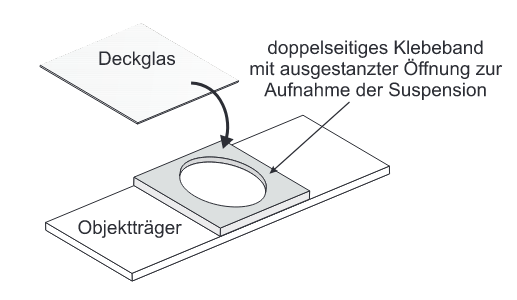
\includegraphics[width=0.48\textwidth]{graphics/probe.png}\label{fig:probe}}
  \hfill
  \caption{Versuchsaufbau [Quelle: PAP2.1 Skript, S.50 (a) \& 54 (b), 08.03.2024]}
  \label{fig:Aufbau}
\end{figure}


%---------------VERSUCHSPROTOKOLL MIT MESSDATEN---------------
\newpage

\section{Versuchsprotokoll mit Messdaten}

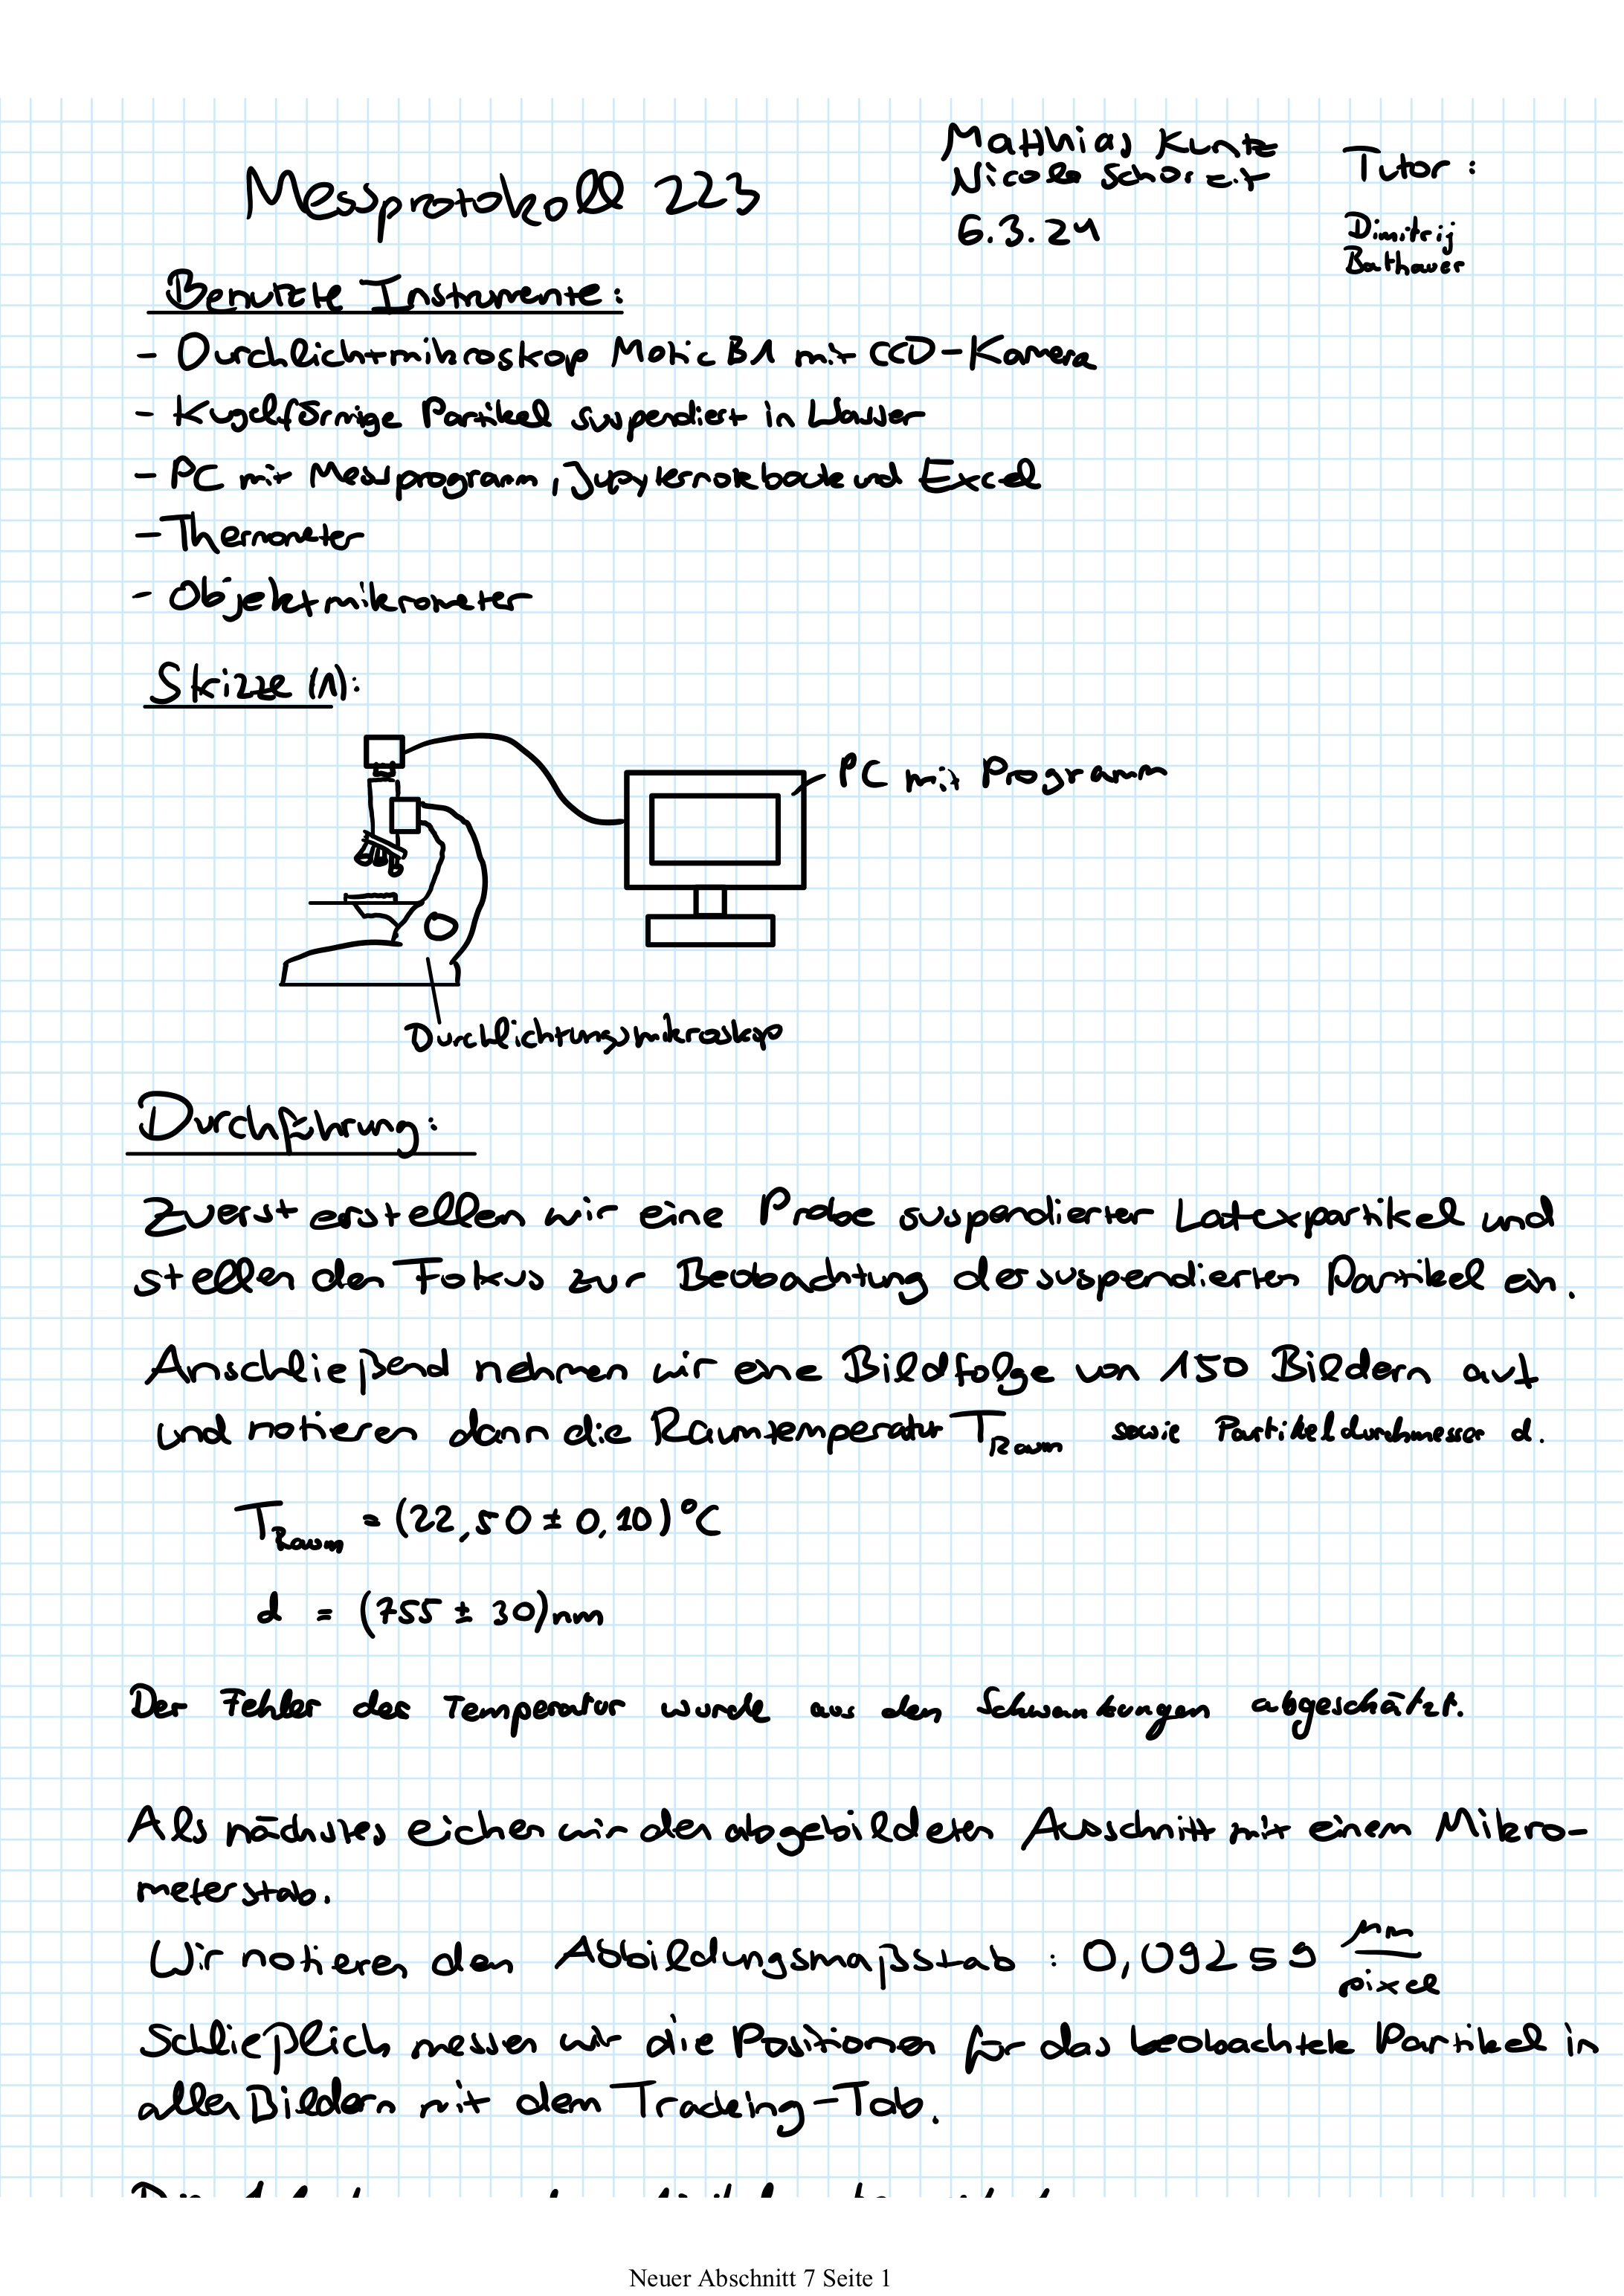
\includegraphics[width=\textwidth]{graphics/mess1.jpg}
\newpage
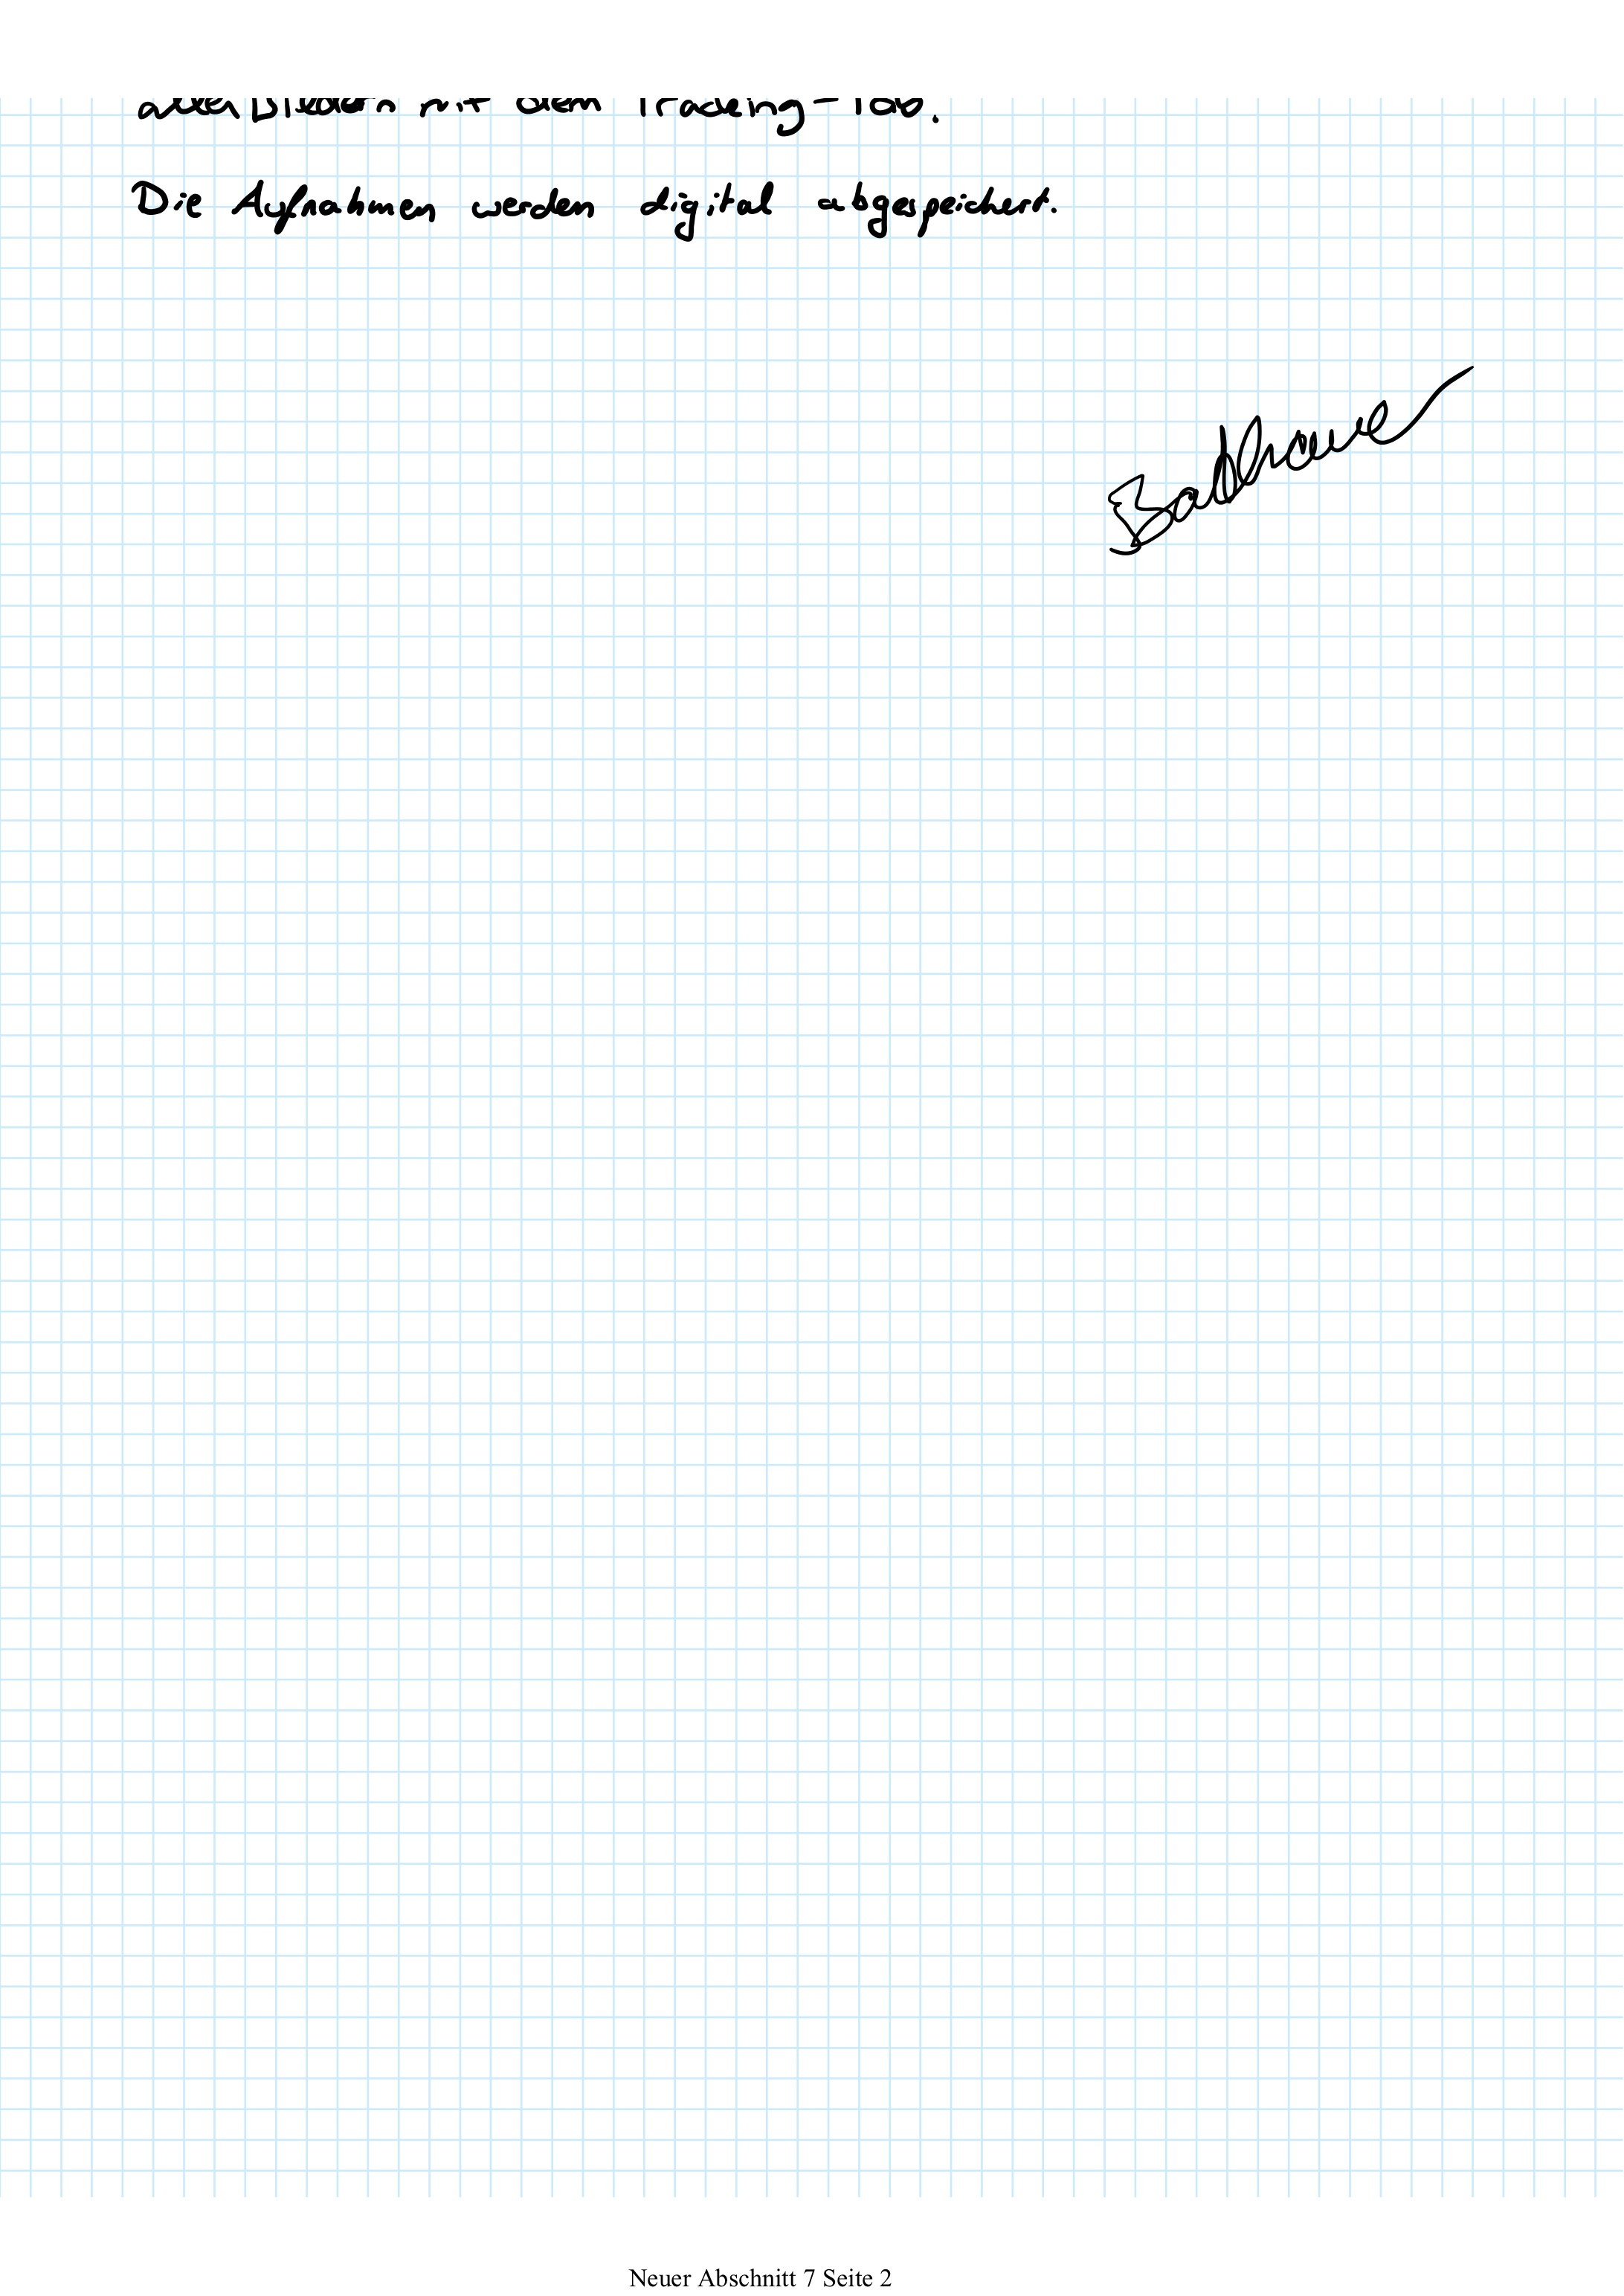
\includegraphics[width=\textwidth]{graphics/mess2.jpg}
\newpage

\begin{figure}[!p]
  \centering
  \subfloat[Beispielaufnahme der beobachteten Teilchen]{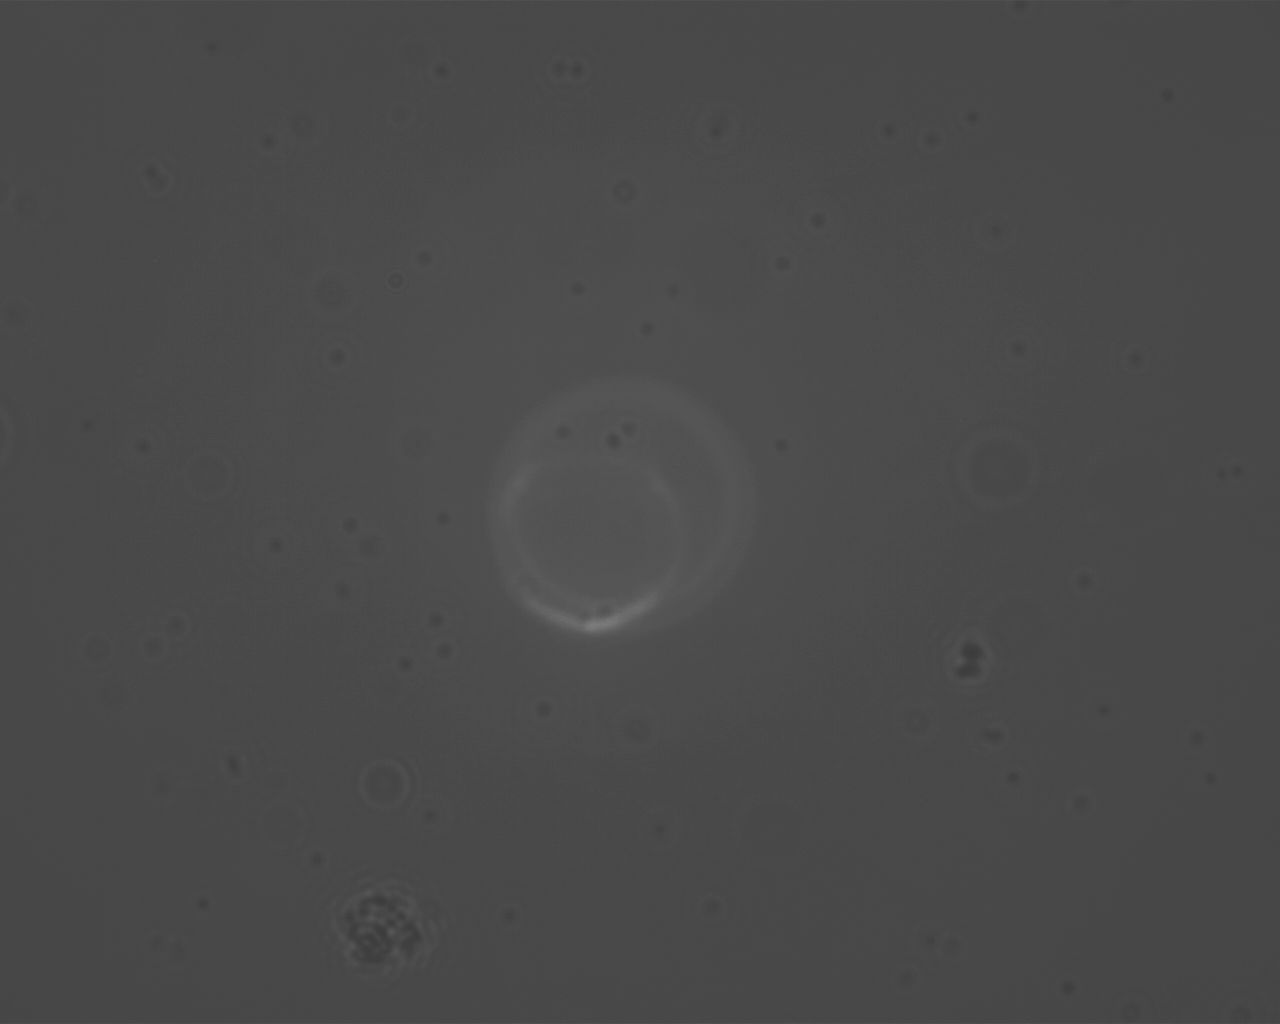
\includegraphics[width=0.9\textwidth]{graphics/Bild0.png}}
  \hfill
  \subfloat[Kalibrierung mit dem Objektmikrometer]{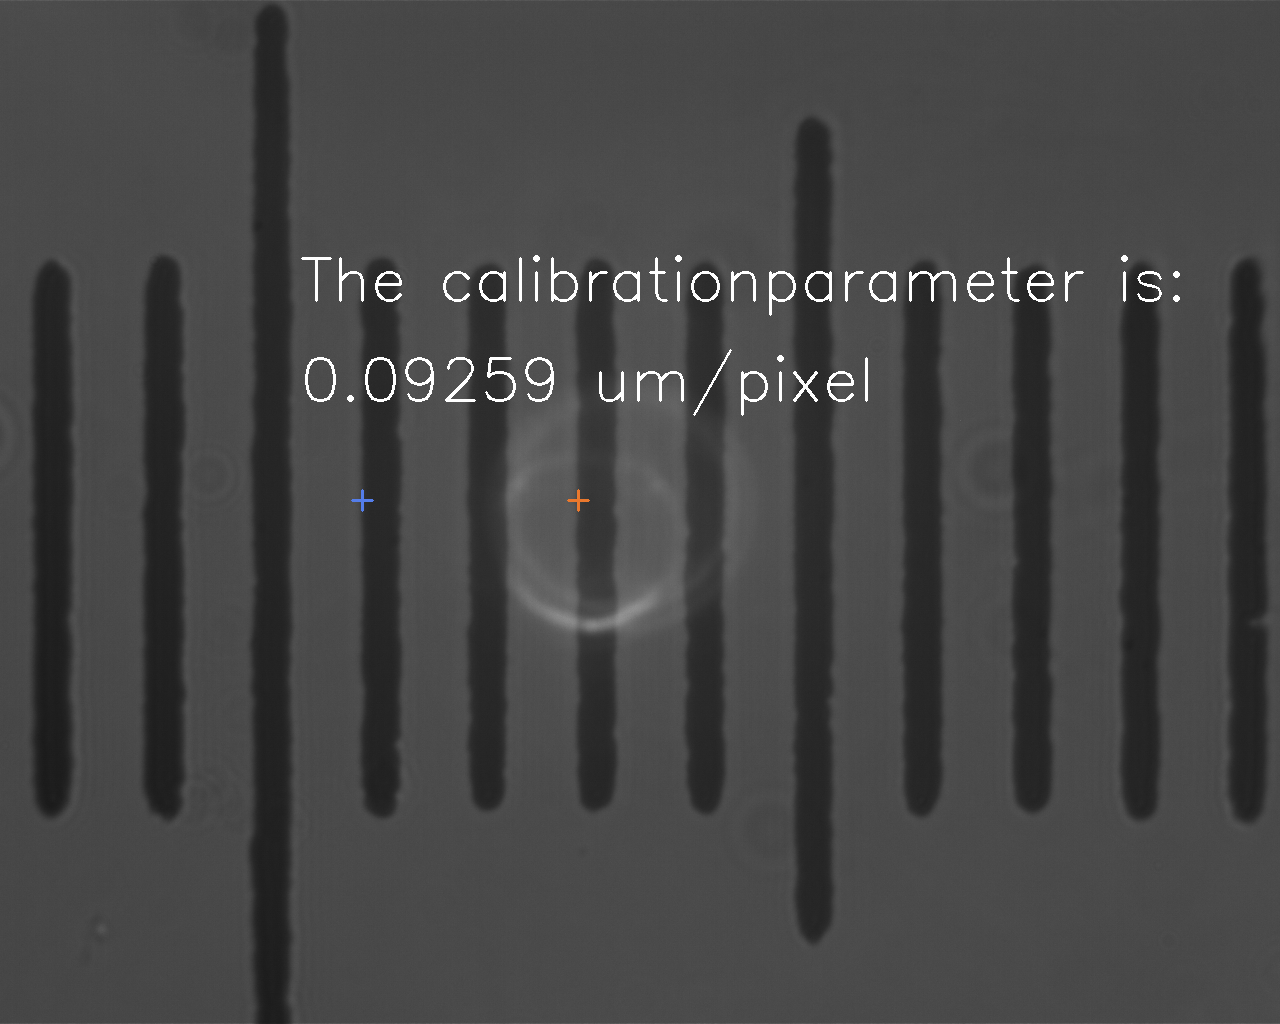
\includegraphics[width=0.9\textwidth]{graphics/Calibration.png}}
  \hfill
  \caption{Bilder der Versuchsdurchführung}
  \label{fig:Durchführung}
\end{figure}

\clearpage
\newpage
%-------------------------AUSWERTUNG-------------------------
\section{Auswertung}

In dieser Evaluation werden alle Fehler, sofern keine spezifische Angabe gemacht wird, mithilfe der Gauss'schen Fehlerfortpflanzung berechnet. Dies bedeutet, dass ein Wert $F$, der mit der Formel $f(a_1, ..., a_n)$ berechnet wird, den Fehler $\Delta F$ annimmt:

\begin{equation}
    \Delta F = \sqrt{\sum_n \left( \frac{\partial f}{\partial a_n} \cdot \Delta a_n \right)^2}.
\end{equation}

Des Weiteren erfolgen Signifikanztests von zwei Werten $a$ und $a'$ über die folgende Formel:

\begin{equation}
    \sigma = \frac{|a-a'|}{\sqrt{(\Delta a)^2 + (\Delta a')^2}}.
\end{equation}

Die Güte eines Fits wird mit der $\chi^2$-Summe bewertet:

\begin{equation}
    \chi^2 = \sum_i^N \left( \frac{\textit{Funktionswert}_i - \textit{Messwert}_i}{\textit{Fehler}_i} \right)^2
\end{equation}

Auch verwendet wird $\chi^2_{red} = \chi^2 / f$, wobei der Freiheitsgrad $f$ die Anzahl der Messwerte minus die Anzahl der Fitparameter ist. Der auf die Freiheitsgrade normierte Wert soll bei einem guten Fit ungefähr 1 sein.

Die Auswertung sowie Berechnung erfolgen über das dem Dokument angehängte Python-Programm.

\newpage

\subsection{Grafische Darstellung der Messdaten} \label{grafisch}

Wir beginnen, indem wir die vom Messprogramm gespeicherten Positionsdaten des beobachteten Teilchens grafisch auswerten. Da wir die Daten der x- und y-Positionen zu jeder Bildaufnahme über 150 Sekunden haben bietet es sich zunächst an, diese Grafisch darzustellen. Dazu erstellen wir ein Diagramm, indem der Weg des Teilchens dargestellt wird, indem alle (x, y)-Paare nacheinander verbunden eingetragen werden. Das Diagramm ist mit zusätzlichen Markern für die Start- und Endposition in Abbildung \ref{fig:brown1} zu sehen.  

Es fällt auf, dass das Teilchen sich immer wieder für längere Zeit in ungefähr dem selben Gebiet aufhält, bevor es dann irgendwann deutlich sichtbar woanders hinläuft. Dies ist vor allem um den Endpunkt der Fall, wo sich das Teilchen für einen längeren Zeitraum in dessen Umgebung befindete. Insgesamt wirkt der Verlauf aber doch sehr zufällig ohne eine deutlich sichtbare Tendenz der Bewegung in eine Richtung, was einen Fluss der Flüssigkeit bedeuten wurde. Somit kann man allein von der grafischen Interpretation annehmen, dass der Verlauf größtenteils auf der zufälligen Brownschen Bewegung basiert.   

\begin{figure}[!h]
    \centering
    \resizebox{0.9\textwidth}{!}{
    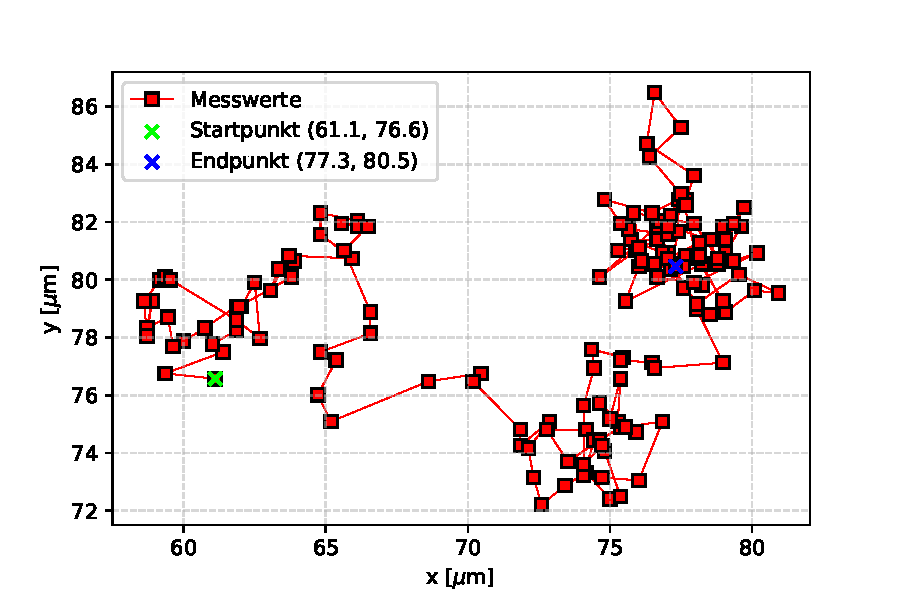
\includegraphics{graphics/brown1-2.pdf}}
    \caption{Aufgenommene Bewegung eines Partikels}
    \label{fig:brown1}
\end{figure}


\newpage
\subsection{Berechnung vom Mittleren Verschiebungsquadrat} \label{Boltzmann1}

Um das mittlere Verschiebungsquadrat zu bestimmen, berechnen wir zunächst für alle Messwerte die Differenz in x- und y-Richtung $\Delta x \ \& \ \Delta y$ zum nächsten Messwert:

\begin{equation}
    \begin{split}
        \Delta x_i &= x_{i+1} - x_i \\
        \Delta y_i &= y_{i+1} - y_i.
    \end{split}
\end{equation}

Das Verscheibungsquadrat für jeden Schritt ergibt sich nun ganz klassisch nach Pythagoras aus der quadratischen Addition der beiden Werte:

\begin{equation}
     r^2_i = \Delta x_i^2 + \Delta y_i^2.
\end{equation}

Zur groben Übersicht werden die Werte in Tabelle \ref{tab:Verschiebung} eingetragen. Das mittlere Verschiebungsquadrat $\langle r^2 \rangle$ ist nun, wie der Name bereits vermuten lässt, der Mittelwert aller berechneten $r^2_i$. Der Fehler berechnet sich aus dem Standardfehler des Mittelwerts:

\begin{equation}
    \Delta \langle r^2 \rangle = \frac{\sigma_{Std}}{\sqrt{N}} = \sqrt{\frac{1}{N^2} \sum_{i=1}^N (\langle r^2 \rangle - r^2_i)^2}.
\end{equation}

Wir erhalten aus den Messdaten somit:

\begin{equation}
    \langle r^2 \rangle = (1,80 \pm 0,16) \ \mu \text{m}^2.
\end{equation}

Dieser Wert ermöglicht uns nun eine Berechnung der Boltzmann-Konstante $k_B$. Dazu verwenden wir Gleichung \ref{eq:Boltzmann}, wofür wir noch die Viskosität von Wasser benötigen. Um diese zu bestimmen verwenden wir das dem Skript angehängte Diagramm der Viskosität in Abhängigkeit der Temperatur und lesen den Wert bei der von uns aufgenommenen Raumtemperatur $T = (22,5 \pm 1,0)^\circ$C ab, siehe Abbildung \ref{fig:viskos}. Der Fehler wird von unserem Temperaturfehler ausgehend abgeschätzt:

\begin{equation}
    \eta = (9,45 \pm 0,05) \cdot 10^{-4} \ \text{Pa s}.
\end{equation}

\begin{figure}[!h]
    \centering
    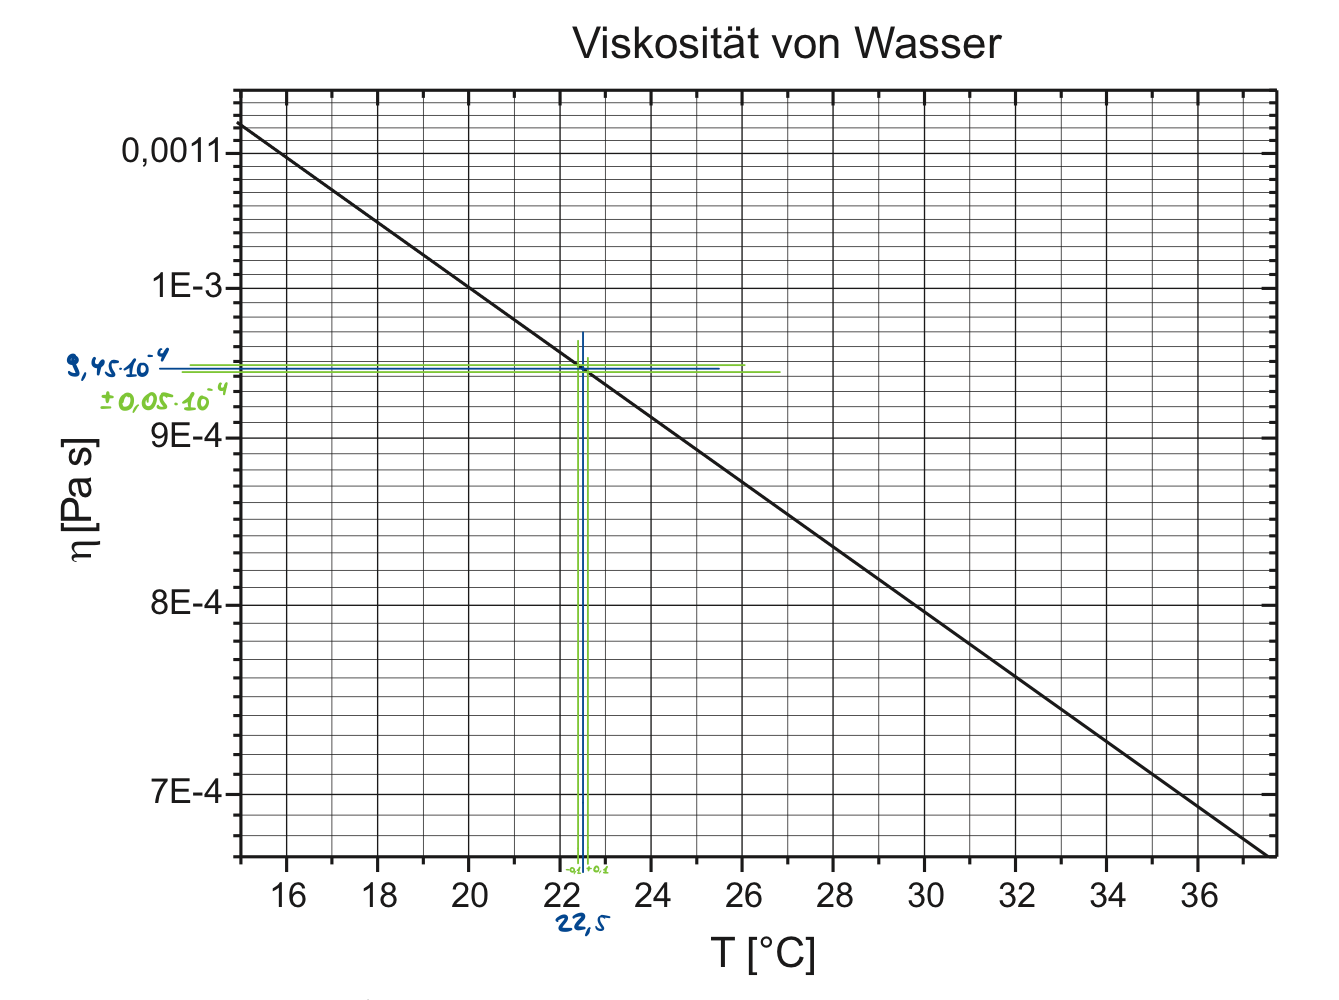
\includegraphics[width=0.9\textwidth]{graphics/viskositaet.png}
    \caption{Temperaturabhängigkeit der Viskosität von Wasser [Quelle: PAP2.1 Skript, S.61, 08.03.2024]}
    \label{fig:viskos}
\end{figure}

\newpage
Wir berechnen nun die Boltzmann-Konstante mit den berechneten Werten sowie dem Wert $2a = (755 \pm 30) \cdot 10^{-9}$m und $T = (295,65 \pm 1,0)$K. Wir setzten, da die Verschiebungen jeweils im Abstand einer Sekunde aufgenommen wurden, $t=1$s.

\begin{equation}
    \begin{split}
            k_B &= \frac{6 \pi \eta a}{4 T t} \langle r^2 \rangle \\
            \Rightarrow \Delta k_B &= k_B \sqrt{\left( \frac{\Delta \langle r^2 \rangle}{\langle r^2 \rangle} \right)^2 + \left( \frac{\Delta \eta}{\eta} \right)^2 +\left( \frac{\Delta T}{T} \right)^2 +\left( \frac{\Delta a}{a} \right)^2} \\ \\
            &\Rightarrow k_{B,1} = (1,03 \pm 0,10) \cdot 10^{-23} \text{J K}^{-1}.
    \end{split}
\end{equation}

Mit diesem Wert können wir nach Gleichung \ref{eq:Einst_Stokes_D} den Diffusionskoeffizienten bestimmen:

\begin{equation}
    \begin{split}
        D &= \frac{k_B T}{6 \pi \eta a} \\
        \Rightarrow \Delta D &= D \sqrt{\left( \frac{\Delta k_B}{k_B} \right)^2 + \left( \frac{\Delta \eta}{\eta} \right)^2 +\left( \frac{\Delta T}{T} \right)^2 +\left( \frac{\Delta a}{a} \right)^2} \\ \\
        &\Rightarrow D_1 = (4,5 \pm 0,5) \cdot 10^{-13} \frac{\text{m}^2}{\text{s}}.
    \end{split}
\end{equation}

Abschließend können wir den berechneten Wert der Boltzmann-Konstante noch mit dem Literaturwert $k_{B,lit} = 1,380649 \cdot 10^{-23} \text{J K}^{-1}$ vergleichen. Hierbei erhalten wir eine Abweichung von $\sigma_{k_1,lit} = 3,6$. Dies ist eine signifikante Abweichung. 

\begin{table}[!p]

\begin{minipage}{0.5\textwidth}
\centering
\resizebox{\textwidth}{!}{
\begin{tabular}{cccc}
\toprule
\textbf{Nr.} & $\bm{dx}$ [$\mu$m] & $\bm{dy}$ [$\mu$m] & $\bm{r^2}$ [$\mu$m$^2$] \\
\midrule
\phantom{\vdots} \\
     1 & -1,76 &  0,19 &  3,13 \\
     2 &  2,04 &  0,74 &  4,7  \\
     3 & -0,37 &  0,28 &  0,21 \\
     4 &  0,83 &  0,46 &  0,91 \\
     5 &  0    &  0,83 &  0,69 \\
     6 & -1,11 & -0,74 &  1,78 \\
     7 & -0,74 & -0,46 &  0,76 \\
     8 & -0,37 & -0,19 &  0,17 \\
     9 & -0,19 &  1,02 &  1,07 \\
    10 & -0,74 & -0,37 &  0,69 \\
    11 &  0,19 &  0,93 &  0,89 \\
    12 & -0,19 & -1,2  &  1,48 \\
    13 & -0,09 &  1,2  &  1,46 \\
    14 &  0,56 &  0,74 &  0,86 \\
    15 &  0,19 &  0,09 &  0,04 \\
    16 &  0,19 & -0,09 &  0,04 \\
    17 &  2,31 & -1,39 &  7,29 \\
    18 &  0,83 & -0,65 &  1,11 \\
    19 & -0,19 &  1,94 &  3,81 \\
    20 & -0,46 & -0,83 &  0,91 \\
    21 & -0,09 &  0    &  0,01 \\
    22 &  1,85 &  1,02 &  4,47 \\
    23 &  0,09 &  0,56 &  0,32 \\
    24 & -0,56 & -0,28 &  0,39 \\
    25 & -0,28 & -0,74 &  0,63 \\
    26 &  0,65 &  1,2  &  1,87 \\
    27 &  2,22 & -0,09 &  4,95 \\
    28 & -1,11 &  0,83 &  1,93 \\
    29 &  0    &  0,74 &  0,55 \\
    30 &  1,3  & -0,28 &  1,76 \\
    31 &  0    & -0,19 &  0,03 \\
    32 & -0,56 &  0,09 &  0,32 \\
    33 &  0,93 & -0,09 &  0,87 \\
    34 & -0,83 & -0,83 &  1,39 \\
    35 &  0,93 & -2,13 &  5,39 \\
    36 &  0    & -0,74 &  0,55 \\
    37 & -1,76 & -0,65 &  3,51 \\
    38 &  0,56 & -0,28 &  0,39 \\
    39 & -0,65 & -1,2  &  1,87 \\
    40 &  0,46 & -0,93 &  1,07 \\
\vdots & \vdots & \vdots & \vdots  \\ 
\bottomrule
\end{tabular}}

\end{minipage} \hfill
\begin{minipage}{0.5\textwidth}
\centering
\resizebox{\textwidth}{!}{
\begin{tabular}{cccc}
\toprule
\textbf{Nr.} & $\bm{dx}$ [$\mu$m] & $\bm{dy}$ [$\mu$m] & $\bm{r^2}$ [$\mu$m$^2$] \\
\midrule
\vdots & \vdots & \vdots & \vdots  \\ 
    41 &  3,43 &  1,39 & 13,67 \\
    42 &  1,85 &  0,28 &  3,51 \\
    43 & -0,28 & -0,28 &  0,15 \\
    44 &  1,67 & -1,67 &  5,56 \\
    45 &  0    & -0,56 &  0,31 \\
    46 &  1,02 &  0,83 &  1,73 \\
    47 & -0,74 & -0,93 &  1,41 \\
    48 &  0,19 & -1,02 &  1,07 \\
    49 &  0,28 & -0,93 &  0,93 \\
    50 &  0,83 &  0,65 &  1,11 \\
    51 &  0,74 &  0,46 &  0,76 \\
    52 &  0,83 & -0,93 &  1,55 \\
    53 &  0,37 &  0,09 &  0,15 \\
    54 & -0,56 &  1,57 &  2,79 \\
    55 & -0,65 &  0,74 &  0,97 \\
    56 & -1,39 &  0    &  1,93 \\
    57 &  0,74 & -1,11 &  1,78 \\
    58 &  1,85 &  1,2  &  4,88 \\
    59 & -0,74 &  0,83 &  1,24 \\
    60 &  0,65 & -0,65 &  0,84 \\
    61 &  0,09 &  1,48 &  2,2  \\
    62 & -0,37 & -1,39 &  2,07 \\
    63 &  0,93 & -0,46 &  1,07 \\
    64 & -0,37 &  0,19 &  0,17 \\
    65 &  1,3  &  0,19 &  1,71 \\
    66 & -0,83 & -2,04 &  4,84 \\
    67 & -1,3  &  0,09 &  1,69 \\
    68 & -0,65 &  0,09 &  0,43 \\
    69 &  0,37 &  1,2  &  1,59 \\
    70 &  0,19 &  0    &  0,03 \\
    71 &  0,09 & -0,19 &  0,04 \\
    72 & -0,65 & -0,65 &  0,84 \\
    73 &  0    &  2,04 &  4,15 \\
    74 &  0,37 &  1,3  &  1,82 \\
    75 & -0,09 &  0,65 &  0,43 \\
    76 &  1,11 & -0,28 &  1,31 \\
    77 & -0,09 & -0,09 &  0,02 \\
    78 &  1,11 & -0,09 &  1,24 \\
    79 &  0,09 & -0,19 &  0,04 \\
    80 &  2,41 &  0,19 &  5,83 \\
\vdots & \vdots & \vdots & \vdots  \\ 
\bottomrule
\end{tabular}}

\end{minipage}

\end{table}

\begin{table}[!p]

\begin{minipage}{0.5\textwidth}
\centering
\resizebox{\textwidth}{!}{
\begin{tabular}{cccc}
\toprule
\textbf{Nr.} & $\bm{dx}$ [$\mu$m] & $\bm{dy}$ [$\mu$m] & $\bm{r^2}$ [$\mu$m$^2$] \\
\midrule
\vdots & \vdots & \vdots & \vdots  \\ 
    81 & -0,93 &  1,85 &  4,29 \\
    82 &  0,46 & -0,19 &  0,25 \\
    83 &  0,46 &  0,37 &  0,35 \\
    84 & -0,74 &  1,39 &  2,48 \\
    85 & -2,69 & -1,3  &  8,89 \\
    86 &  0,46 &  1,2  &  1,66 \\
    87 &  1,67 &  0,37 &  2,91 \\
    88 & -0,65 &  0,09 &  0,43 \\
    89 & -0,37 &  0,93 &  0,99 \\
    90 & -2,04 & -1,76 &  7,24 \\
    91 &  1,3  &  0,93 &  2,54 \\
    92 &  0,74 &  0,37 &  0,69 \\
    93 & -0,93 &  0    &  0,86 \\
    94 &  1,11 & -0,46 &  1,45 \\
    95 & -0,09 &  1,11 &  1,24 \\
    96 &  0,28 & -0,46 &  0,29 \\
    97 & -1,39 &  0,19 &  1,96 \\
    98 & -0,28 &  0,19 &  0,11 \\
    99 & -0,56 &  0,83 &  1    \\
   100 &  1,67 & -0,46 &  2,99 \\
   101 &  0,93 &  0,46 &  1,07 \\
   102 &  0    & -1,11 &  1,23 \\
   103 & -0,28 & -1,3  &  1,76 \\
   104 &  0,46 & -0,65 &  0,63 \\
   105 & -0,46 &  0,83 &  0,91 \\
   106 &  0,93 & -1,39 &  2,79 \\
   107 &  1,48 &  1,02 &  3,23 \\
   108 &  1,39 & -0,65 &  2,35 \\
   109 & -0,83 &  0,09 &  0,7  \\
   110 & -1,02 & -0,74 &  1,59 \\
   111 & -0,09 &  0,37 &  0,15 \\
   112 & -0,93 &  1,48 &  3,05 \\
   113 & -0,46 &  1,94 &  3,99 \\
   114 &  0,09 &  0,09 &  0,02 \\
   115 &  0,28 &  0,83 &  0,77 \\
   116 & -1,67 &  1,11 &  4,01 \\
   117 &  0,28 &  1,76 &  3,17 \\
   118 &  0,93 & -1,2  &  2,31 \\
   119 & -1,11 & -1,02 &  2,27 \\
   120 &  1,11 & -1,3  &  2,91 \\
\vdots & \vdots & \vdots & \vdots  \\ 
\bottomrule
\end{tabular}}

\end{minipage}
\begin{minipage}{0.5\textwidth}
\centering
\resizebox{\textwidth}{!}{
\begin{tabular}{cccc}
\toprule
\textbf{Nr.} & $\bm{dx}$ [$\mu$m] & $\bm{dy}$ [$\mu$m] & $\bm{r^2}$ [$\mu$m$^2$] \\
\midrule
\vdots & \vdots & \vdots & \vdots  \\ 
   121 & -0,37 & -0,74 &  0,69 \\
   122 &  0,56 &  0,37 &  0,45 \\
   123 & -0,65 & -0,74 &  0,97 \\
   124 &  1,48 & -0,46 &  2,41 \\
   125 &  0,28 & -0,83 &  0,77 \\
   126 &  0,83 &  1,3  &  2,37 \\
   127 & -0,56 & -0,93 &  1,17 \\
   128 & -0,09 &  0,93 &  0,87 \\
   129 & -1,39 & -1,39 &  3,86 \\
   130 & -0,93 & -0,37 &  0,99 \\
   131 &  1,57 & -0,28 &  2,55 \\
   132 & -0,28 &  0,09 &  0,09 \\
   133 &  2,22 &  1,02 &  5,98 \\
   134 & -0,83 & -0,28 &  0,77 \\
   135 & -0,28 &  0,74 &  0,63 \\
   136 &  0,28 &  0,56 &  0,39 \\
   137 &  0,37 &  0,56 &  0,45 \\
   138 & -0,93 & -1,76 &  3,95 \\
   139 & -0,83 &  1,2  &  2,14 \\
   140 & -2,13 &  0,37 &  4,67 \\
   141 &  0,28 & -1,67 &  2,85 \\
   142 & -0,09 &  0,46 &  0,22 \\
   143 & -0,74 & -0,09 &  0,56 \\
   144 &  1,3  & -0,46 &  1,89 \\
   145 &  0,56 & -0,19 &  0,34 \\
   146 &  1,02 &  0,46 &  1,25 \\
   147 &  0    &  0,46 &  0,21 \\
   148 & -1,11 & -0,56 &  1,54 \\
   149 &  0,28 & -0,28 &  0,15 \\
\phantom{\vdots} \\
\phantom{.} \\
\phantom{.} \\
\phantom{.} \\
\phantom{.} \\
\phantom{.} \\
\phantom{.} \\
\phantom{.} \\
\phantom{.} \\
\phantom{.} \\
\phantom{.} \\
\phantom{.} \\
\bottomrule
\end{tabular}}

\end{minipage}

\caption{Berechnung Verschiebungen}
\label{tab:Verschiebung}
\end{table}


\clearpage
\newpage

\subsection{Kontrollverteilung} \label{Hist}

Wir wollen nun überprüfen, ob unsere Annahmen in der Vorbereitung akzeptabel waren. Dazu überprüfen wir, ob die gemessenen Verschiebungen tatsächlich Gaußverteilt sind. Wir betrachten also alle bestimmten $dx$ und $dy$ und tragen diese in ein Histogramm ein. Da die Brownsche Bewegung isotrop ist, können wir das einfach machen und müssen nicht spezifisch zwischen den Richtungen der Verschiebung unterteilen. Zusätzlich normieren wir das Histogramm auf die relative Häufigkeit. Wenn wir alles richtig gemacht haben, sollte die Verteilung nun Gaußförmig aussehen. Zum Vergleich plotten wir die Gaußverteilung über das Histogramm, die sich aus dem Mittelwert aller Verschiebungen $\mu_{dx,dy}$ sowie dessen Standardabweichung $\sigma_{dx,dy}$ ergibt:

\begin{equation}
    G(x; \ \mu_{dx,dy}, \ \sigma_{dx,dy}) = \frac{1}{\sqrt{2 \pi} \sigma_{dx,dy}} \ \exp{\left( - \frac{(x-\mu_{dx,dy})^2}{2\sigma_{dx,dy}^2} \right)}
\end{equation}

Wir erhalten das in Abbildung \ref{fig:brown2} dargestellte Diagramm mit den folgenden Werten:

\begin{equation}
    \begin{split}
        \mu_{dx,dy} &= 0,067 \\
        \sigma_{dx,dy} &= 0,947.
    \end{split}
\end{equation}


Es ist zu erkennen, dass die Verteilung und die Gaußkurve allgemein gut übereinanderliegen. Allein im Bin direkt unterhalb der 0 ist eine deutliche Abweichung von der Gaußverteilung zu beobachten. Abgesehen davon sieht man den erwarteten Abfall an den Seiten, wo Kurve und Histogramm in beiden Richtung sehr gut zusammenpassen. Wir können also schlussfolgern, dass unsere vermessene Bewegung annähernd Gaußverteilt ablief.

\begin{figure}[!hp]
    \centering
    \resizebox{0.9\textwidth}{!}{
    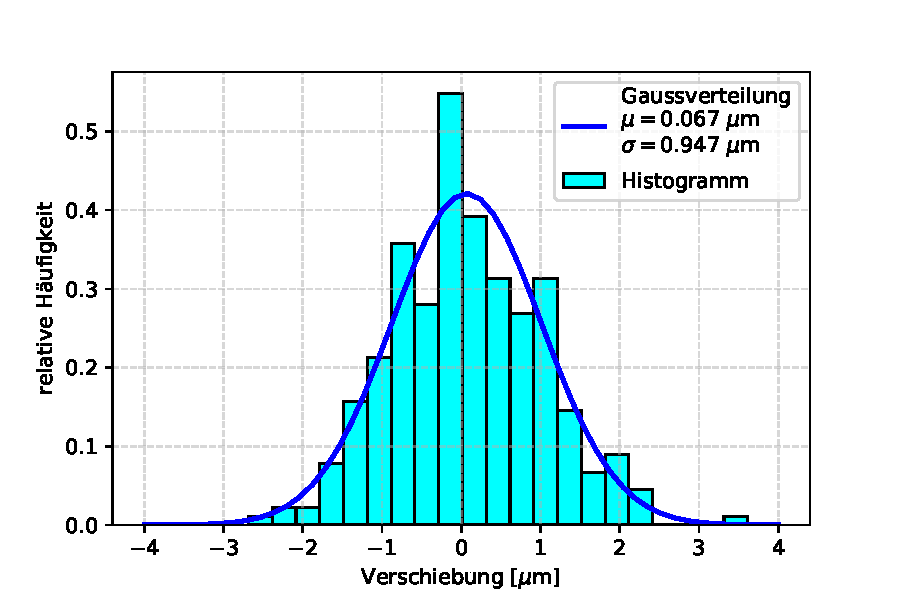
\includegraphics{graphics/brown2.pdf}}
    \caption{Histogramm der Verschiebungen mit Gaußkurve}
    \label{fig:brown2}
\end{figure}


\clearpage
\newpage
\subsection{Kumulative Verteilung der Verschiebungsquadrate}

Zu guter Letzt wollen wir erneut Diffusionskoeffizient und Boltzmann-Konstante mithilfe einer anderen Methode berechnen. Betrachten wir die Einstein-Smolu-chowski-Gleichung für 2 Dimensionen, Gleichung \ref{eq:r^2_2dim}, so stellt man fest, dass sich der Diffusionskoeffizient $D$ aus der Steigung einer Geraden des aufaddierten mittleren Verschiebungsquadrats als Funktion der Zeit ergibt. Wir tragen also mit diesem Ziel die kumulative Summe der Verschiebungsquadrate gegen die Zeit in eine Diagramm auf und fitten eine lineare Funktion $y = ax+b$ an. Den Fit übernimmt Python für uns und bestimmt dabei als beste Werte:

\begin{equation}
    \begin{split}
        a = 4D &= (1,870 \pm 0,007) \ \frac{\mu \text{m}^2}{\text{s}}, \\
        b &= -(2,0 \pm 0,6) \ \mu \text{m}^2.
    \end{split}
\end{equation}

Das Diagramm mit den Werten und eigetragenem Fit ist in Abbildung \ref{fig:brown3} zu sehen. Wir erhalten nach dieser Methode also den Wert:

\begin{equation}
    D_2 = (4,675 \pm 0,018) \cdot 10^{-13} \ \frac{\text{m}^2}{\text{s}}.
\end{equation}

Verwenden wir nun Gleichung \ref{eq:Einst_Stokes_D}, so können wir erneut die Boltzmann-Konstante bestimmen:

\begin{equation}
    \begin{split}
        k_B &= \frac{6 D \pi \eta a}{T} \\
        \Delta k_B &= k_B \sqrt{\left( \frac{\Delta D}{D} \right)^2 + \left( \frac{\Delta \eta}{\eta} \right)^2 +\left( \frac{\Delta T}{T} \right)^2 +\left( \frac{\Delta a}{a} \right)^2} \\ \\
        &\Rightarrow k_{B,2} = (1,06 \pm 0,04) \cdot 10^{-23} \text{J K}^{-1}
    \end{split}
\end{equation}

Wir vergleichen erneut mit dem Literaturwert und erhalten die Abweichung $\sigma_{k_2,lit} = 7,4$. Erneut ist dies eine signifikante Abweichung. 

Analog vergleichen wir noch Diffusionskoeffizient und Boltzmann-Konstante mit den zuvor in Kapitel \ref{Boltzmann1} bestimmten Werten. Hier erhalten wir Abweichungen von $\sigma_D = 0,3$ und $\sigma_{k_B} = 0,3$. Diese Abweichungen sind nicht signifikant, was bedeutet, dass die zwei Methoden miteinander verträgliche Ergebnisse liefern. Die großen Abweichungen im Vergleich mit dem Literaturwert kommen also nicht von einem Fehler in der Auswertungsmethode, sondern müssen stattdessen das Resultat eines grundlegenderen systematischen Fehlers sein.  

\begin{figure}[!hp]
    \centering
    \resizebox{0.9\textwidth}{!}{
    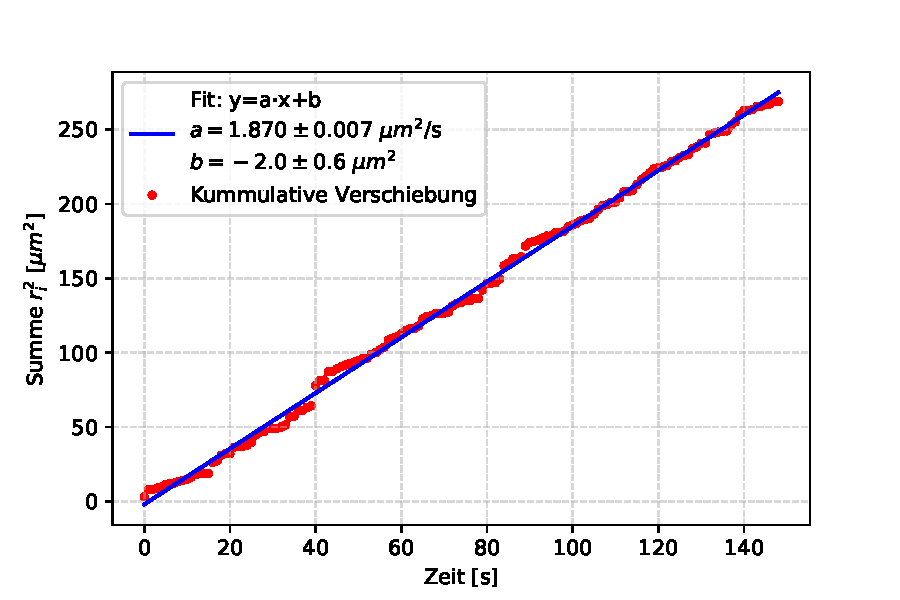
\includegraphics{graphics/brown3.pdf}}
    \caption{Kumulative Verschiebung des Partikels mit Linearem Fit}
    \label{fig:brown3}
\end{figure}

\clearpage
\newpage
%---------------PRÄSENTATION DER ENDERGEBNISSE---------------
\section{Zusammenfassung der Endergebnisse}

Wir begannen mit einer grafischen Analsyse der Bewegung. Es zeigte sich ein sehr zufällig erscheinender Verlauf, wodurch geschlussfolgert wurde, dass tatsächlich eine Brownsche Bewegung ohne deutliche Störungen, wie beispielsweise einem Fluss, vorliegt.

Daraufhin berechnet wir zum ersten Mal den Diffunsionskoeffizienten sowie die Boltzmann-Konstante, indem wir das mittlere Verschiebungsquadrat der Partikelbewegungen pro Sekunde bestimmten. Wir erhielten dabei die folgenden Werte:

\begin{equation}
    \begin{split}
        \langle r^2 \rangle &= (1,80 \pm 0,16) \ \mu \text{m}^2, \\
        k_{B,1} &= (1,03 \pm 0,10) \cdot 10^{-23} \text{J K}^{-1}, \\
        D_1 &= (4,5 \pm 0,5) \cdot 10^{-13} \frac{\text{m}^2}{\text{s}}.
    \end{split}
\end{equation}

Beim Vergleich mit dem Literaturwert der Boltzmann-Konstante ergab sich hier eine signifikante Abweichung von $\sigma_{k_1,lit} = 3,6$.

Anschließend verglichen wir die Verteilung der Verschiebungen mit dem erwarten Gaußförmigen Verlauf. Hier konnten deutliche Parallelen zwischen der gemessenen Verteilung und der theoretischen Gaußverteilung beobachtet werden, allerdings auch eine deutlich erhöhte Anzahl Messungen im Bereich leicht unterhalb des Mittelwerts. 

Zuletzt bestimmten wir erneut den Diffusionskoeffizienten und die Boltzmann-Konstante, diesmal über die kumulative Summe der Verschiebungen mithilfe der Einstein-Smoluchowski-Gleichung. Wir berechnet hier:

\begin{equation}
    \begin{split}
        k_{B,2} &= (1,06 \pm 0,04) \cdot 10^{-23} \text{J K}^{-1}, \\
        D_2 &= (4,675 \pm 0,018) \cdot 10^{-13} \ \frac{\text{m}^2}{\text{s}}.
    \end{split}
\end{equation}

Erneut ergab der Literaturwert-Vergleich eine signifikante Abweichung von diesmal $\sigma_{k_2,lit} = 7,4$. Die Vergleiche mit den zuvor berechneten Werten ergaben allerdings insignifikante Abweichungen von $\sigma_D = 0,3$ und $\sigma_{k_B} = 0,3$.

\newpage
%---------------ZUSAMMENFASSUNG UND DISKUSSION---------------
\section{Diskussion}

Das wohl auffälligste Ergebnis dieses Versuchs sind die hohen Abweichungen der berechneten Boltzmann-Konstanten im Vergleich zum Literaturwert. Doch bevor wir ausführlicher überlegen, woran das gelegen haben mag, möchten wir zuerst mal zusammenfassen was alles gut funktioniert hat. Angefangen bei der grafischen Auswertung konnte ein erwarteter schön zufälliger Verlauf des Teilchens ohne klar sichtbaren Fluss beobachtet werden. Analog lieferte der grafische Vergleich der Verschiebungsverteilung mit dem Gauß eine zufriedenstellende Überlagerung, die bis auf einen kleineren Bereich nicht weiter auffällig war. Auch zeigte die kumulierte Verschiebung den erwarteten linearen Verlauf. Zudem ist es sehr erfreulich, dass die Ergebnisse der verschiedenen Versuchsteile an sich sehr gut zusammenpassen und zueinander beide insignifikante Abweichungen innerhalb der $1\sigma$-Umgebung aufweisen. Auch sind die erhaltenen Ergebnisse der Boltzmann-Konstanten zumindest in der richtigen Größenordnung wie der Literaturwert, was doch auch ein schonmal nicht allzu erschreckendes Ergebnis ist. 

Aber dennoch sind die Abweichungen mit ungefähr 3,6 und 7,4 signifikant und lassen wie bereits erwähnt auf einen grundlegenden systematischen Fehler schließen. Hier ist es sinnvoll zu erwähnen, dass bei der Versuchsdurchführung zuerst eine Probe präpariert wurde, die ein sehr unerwartetes Bild lieferte: Es bewegten sich praktische keine der im Mikroskop aufgelösten Teilchen. Bei einer zweiten präparierten Probe waren zwar deutliche Bewegungen zu erkennen, jedoch war immer noch eine sehr viel höher als eigentlich gedachte Anzahl fast komplett ruhiger Teilchen vorhanden, an manchen Stellen sogar mehr als die Hälfte im Bildausschnitt. Ob hier Mängel an der Probe oder sonstige andere Einflüsse eingewirkt haben können wir schwer beurteilen, aber es ist durchaus möglich, dass an genau diesem Punkt ein Grund für die hohen Abweichungen verborgen liegt. \\ Analog könnte das Problem aber auch in der Bewegung des beobachteten Partikels liegen. Wie in Kapitel \ref{Hist} angemerkt ist eine deutlich höhere Anzahl an Verschiebungen um den Nullwert detektiert worden als eigentlich erwartet. Dies wird auch die Erklärung für die in Kapitel \ref{grafisch} gemachte Beobachtung sein, dass das Teilchen sich häufig viel um eine Stelle herum bewegt, bevor es mal weiter weg wandert. Es wirkt durchaus plausibel, dass der Überschuss an vielen kleineren Bewegungen das Resultat irgendeiner äußeren Beeinflussung der Brownschen Bewegung des Partikels war, die sich im Endeffekt auch auf die berechneten Werte ausgewirkt hat. Erneut ist es schwer zu sagen, woher genau diese untypische Bewegungsweise stammt, da die Bewegung eines Partikels im allgemeinen nunmal sehr komplex ist und auch die in den Grundlagen erklärte Brownsche Bewegung nur auf dem Modell des Random-Walks basierte, was zwar durchaus ein sehr gutes, aber eben kein perfektes Modell darstellt. Eine Idee wäre, dass nicht nur die Zusammenstöße mit den Wassermolekülen die Bewegung des betrachteten Latexpartikels beeinflusste, sondern dieses noch mit irgendwelchen anderen Teilchen oder externen Kräften wechselwirkte. Das ist aber nur eine Vermutung und muss in dieser Form durchaus nicht korrekt sein. \\ Es kann natürlich im Allgemeinen auch sein, dass trotz bestem Gewissen unsererseits auch Fehler bei der Messung Grund für die hohen Abweichungen sein können. Die hohe Empfindlichkeit der Probe auf äußere Erschütterungen oder thermische Veränderungen können Unachtsamkeiten der im Raum anwesenden Personen amplifiziert und im Endeffekt schlagkräftig genug gemacht haben, dass die Ergebnisse so weit verschoben wurden. Aber auch allgemeine Schwankungen der Raumtemperatur oder Erschütterungen im Gebäude von anderweitigen Quellen können die Messungen beeinflusst haben. \\ Auch generelle Objektfehler des verwendeten Mikroskops oder der genutzten Software könnten Grunde sein, jedoch macht nichts außer den Endergebnisse dieses Versuchs den Anschein darauf, weshalb der Fehler unseren Erachtens eher woanders liegen muss.  

Somit lässt sich schlussfolgern, dass sich irgendwo im beim Versuch ein Fehler eingeschlichen hat. Unserer Vermutung nach ist es am wahrscheinlichsten, dass dies bei der Brownschen Bewegung selbst liegt, die bei uns nicht perfekt und nicht garantiert ohne äußere Einflüsse war.

Verbesserungsmöglichkeiten des Versuchs wären somit eventuell die Vermessung von nicht nur einem Teilchen bei nicht nur bei einer Probe. So könnten zwar Teilchen- und Probendifferenzen ausgeglichen, jedoch zugleich vermutlich auch der Rahmen des Anfängerpraktikums gesprengt werden. Auch eine thermische und bewegungsdämmende Isolierung des Mikroskops mit Probe hätte ähnliche positive, aber zugleich ausmaßintensive Effekte.  

Zusammenfassend lässt sich aber sagen, dass trotz der hohen Abweichung vom Literaturwert insgesamt Ergebnisse erzieht wurden, die größtenteils mit der theoretisch Erwartung übereinstimmen, miteinander gut verträglich sind und zumindest in derselben Größenordnung wie die Theorie landen. Somit war der Versuch insgesamt mehr eine interessante und lehrreiche Einführung zur Brownschen Bewegung mit neuen Erfahrungen beim Umgang mit Mikroskopen beziehungsweise generell optischen Systemen.

\newpage
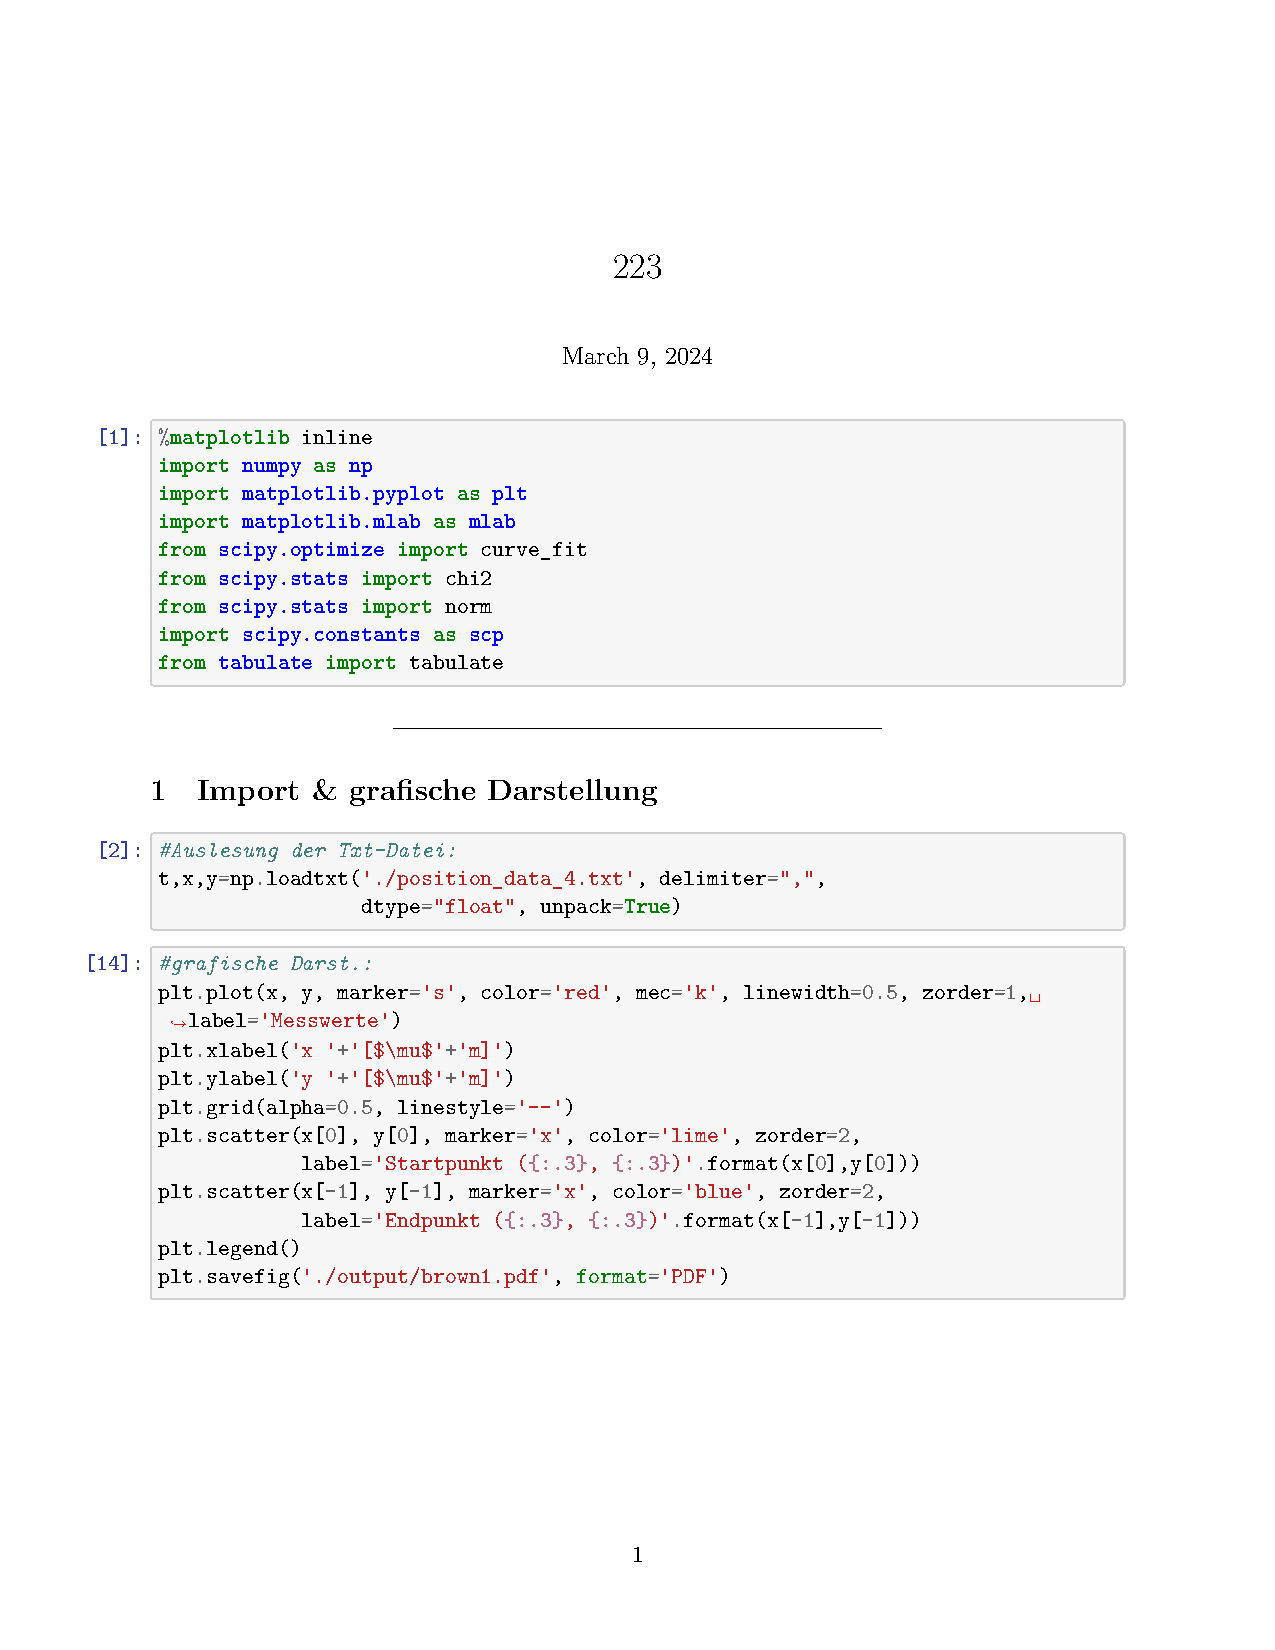
\includepdf[pages=-]{223.pdf}

\end{document}

